\section{Process vs thread}
A comparison is provided in Table \ref{tab:thread_vs_process}.
\begin{table}[h]
	\centering
	\resizebox{\textwidth}{!}{%
		\begin{tabular}[\footnotesize]{|m{\textwidth/8}|m{\textwidth/8}|m{\textwidth/6}|m{\textwidth/8}|m{\textwidth/8}|m{\textwidth/5}|}
			\hline
			& \textbf{Memory} & \textbf{Communication} & \textbf{Creation} & \textbf{Control} & \textbf{Changes} \\ \hline
			\textbf{Thread} & Shared address space between threads & Threads can easily communicate between each other via the shared variables & Threads are easily created and destroyed & Threads can exercise considerable control over threads of the same process & Changes to the main thread (cancellation, priority change, etc.) may affect the behavior of the other threads of the process \\ \hline
			\textbf{Process} & Independent address space between processes & Proesses can communicate via considerable overhead with O.S. interprocess communication & Processess require duplication of the parent process & Processes can only exercise control over child processes. & Changes to the parent process do not affect child processes \\ \hline
		\end{tabular}%
	}
	\caption{Thread vs processes}
	\label{tab:thread_vs_process}
\end{table}

\begin{figure}[]
	\centering
	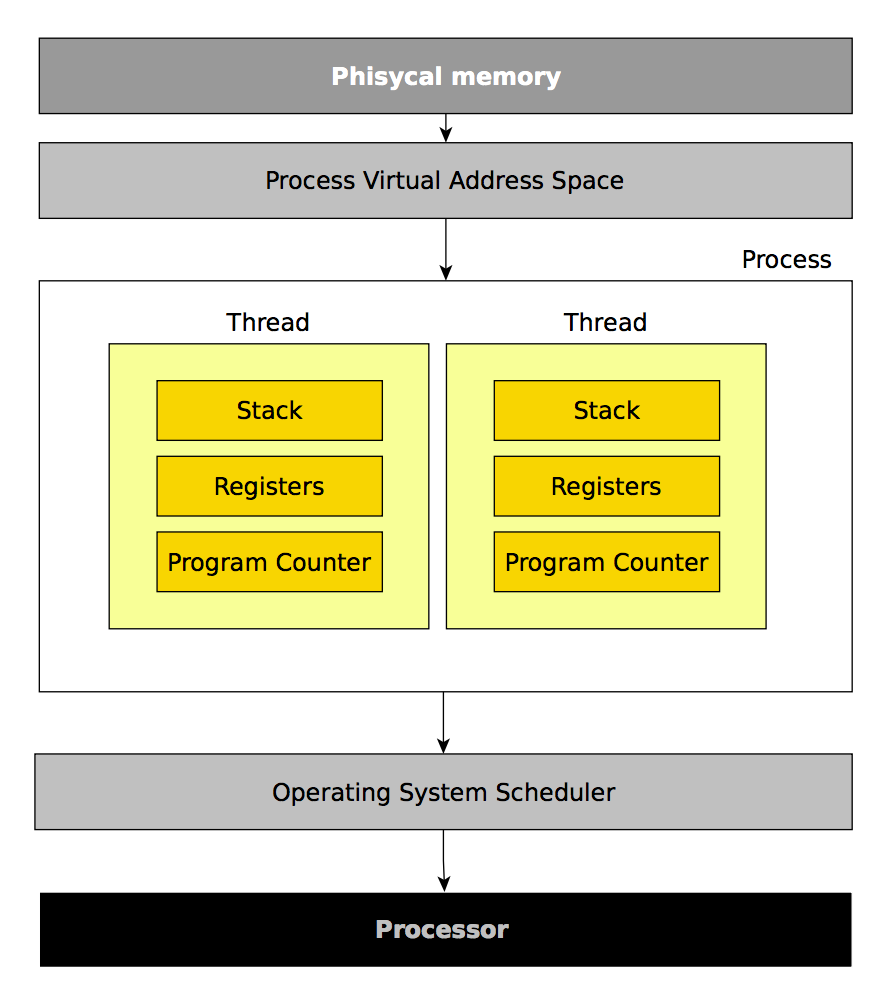
\includegraphics[width=\textwidth]{gfx/process_threads}
	
	\caption{Threads in a process}
	\label{Fig:process_threads}
\end{figure}



\pagebreak

\section{Operations on processes}

\subsection{fork()}
This command creates a process by duplicating the calling process.
\begin{lstlisting}[language=C]
int main()
{
	pid_t child_pid; 

	child_pid = fork();

	if (child_pid != 0)
		printf("Parent: child's process id = %d\n", child_pid);
	else
		printf("Child: my process id = %d\n", (int) getpid()); 
		
	return 0;
}
\end{lstlisting}

When forking a process:
\begin{itemize}
	\item Parent process virtual address space is replicated in the child, Including the states of variables, mutexes, condition variables, POSIX objects.
	\item The child inherits copies of the parent's set of open file descriptors, as well as status fags and current file offset.
\end{itemize}

\subsection{wait()}
The \code{wait(NULL)} waits for a child to end its execution, because the signal \code{NULL} is the one that tells "execution ended". 

This program writes on the stout the child's sentence and then the father's sentence, because he waits for it.
\begin{lstlisting}[language=C]
int main()
{
	pid_t child_pid=0;
	
	child_pid= fork();
	
	wait(NULL);
	
	if(child_pid)
		printf("\nFather's id: %d \n",getpid());
	else
		printf("\nChil's id: %d, with father: %d\n",getpid(),getppid());

	return 0;
}

\end{lstlisting}

\subsection{Signal}
Between processes one can use \code{signals}, that signal an event to a specific PID.
To issue a \code{signal}, we need the function (or the command) \code{kill(pid_t pid,int signal);}.

To listen to a signal we need a \code{struct sigaction}, in where we write the function to be called when the signal is issued, and a \code{sigaction(int signum, const struct sigaction *act, struct sigaction *oldact)} in which we bind the signal issued by the \code{kill} to the function \code{*act}.


\subsection{Pipe}
The pipes can be:
\begin{itemize}
	\item unnamed: useful to exchange data between two forked processes
	\item named: useful to exchange data between two uncorrelated processes. 
\end{itemize}

\subsubsection{Unnamed pipes}
 Unnamed pipes use a shared variable in which a process adds data from one side and the other extracts it from the other side.

\begin{lstlisting}[language=C]
#include <stdlib.h>
#include <stdio.h>
#include <unistd.h>

void writer(const char * message, int count, FILE * stream)
{
	for(; count > 0; --count)
	{
		fprintf(stream, "%s\n", message);
		fflush(stream);
		sleep(1);
	}
}


void reader(FILE * stream)
{
	char buffer[1024];
	while(!feof(stream) && !ferror(stream) && fgets(buffer,
		sizeof(buffer), stream) != NULL)
	fputs(buffer, stdout);
}


int main()
{
	FILE * stream;
	int fds[2]; //the vector that stores the start and the end of the pipe
	pipe(fds);
	pid_t pid = fork();
	/* Child process (consumer) */
	if(pid == (pid_t) 0)
	{
		close(fds[1]);
		/* Close the copy of the fds write end */
		stream = fdopen(fds[0], "r");
		reader(stream);
		close(fds[0]);
	}
	else
	{
		close(fds[0]);
		/* Close the copy of the fds read end */
		stream = fdopen(fds[1], "w");
		writer("Hello, world.", 3, stream);
		close(fds[1]);
	}
	
	return 0;

}
\end{lstlisting}

\subsubsection{Named pipes}
Use a file to exchange data.




